\documentclass[conference]{IEEEtran}
\IEEEoverridecommandlockouts
% The preceding line is only needed to identify funding in the first footnote. If that is unneeded, please comment it out.
%Template version as of 6/27/2024

\makeatletter
\newcommand{\linebreakand}{%
  \end{@IEEEauthorhalign}
  \hfill\mbox{}\par
  \mbox{}\hfill\begin{@IEEEauthorhalign}
}
\makeatother

\usepackage{cite}
\usepackage{amsmath,amssymb,amsfonts}
\usepackage{algorithmic}
\usepackage{graphicx}
\usepackage{textcomp}
\usepackage{xcolor}
\usepackage{hyperref}
\usepackage{textcomp}
\usepackage{makecell} 
\usepackage{array}
\usepackage{tabularx}   % add this in preamble
\usepackage{amssymb}    % for \checkmark




\def\BibTeX{{\rm B\kern-.05em{\sc i\kern-.025em b}\kern-.08em
    T\kern-.1667em\lower.7ex\hbox{E}\kern-.125emX}}
\begin{document}

\title{Benchmarking Distributed SQL Query Execution with PrestoDB}

\author{\IEEEauthorblockN{Emmanouil Pantelakis}
    \IEEEauthorblockA{\textit{School of Electrical and Computer Engineering} \\
        \textit{National Technical University of Athens}\\
        Athens, Greece \\
        el20853@mail.ntua.gr}
    \and
    \IEEEauthorblockN{Ioannis Dimoulas}
    \IEEEauthorblockA{\textit{School of Electrical and Computer Engineering} \\
        \textit{National Technical University of Athens}\\
        Athens, Greece \\
        el20083@mail.ntua.gr}
    \linebreakand
    \IEEEauthorblockN{Enrica Iliana Maggiori}
    \IEEEauthorblockA{\textit{School of Electrical and Computer Engineering} \\
        \textit{National Technical University of Athens}\\
        Athens, Greece \\
        el20143@mail.ntua.gr}
}

\maketitle

\begin{abstract}
    Some abstract text
\end{abstract}

\begin{IEEEkeywords}
    PrestoDB, Big Data, Distributed SQL Queries
\end{IEEEkeywords}

\section{Introduction}


\section{System Architecture and Software Description}\label{SystemArchitecture}

\subsection{Infrastructure Description}

For the purposes of our project, we were provided with two virtual machines by okeanos-knossos, a GRNET's IaaS cloud service for the Greek Research and Academic Community\cite{b1}.
The specifications of each virtual machine are as follows:

\begin{itemize}
    \item \textbf{CPU:} 8 virtual cores - Intel(R) Xeon(R) CPU E5-2650 v3
    \item \textbf{RAM:} 16 GB
    \item \textbf{Storage:} 60 GB (30 GB SSD plus an additional 30 GB of attached storage)
    \item \textbf{Operating System:} Ubuntu Server 24.04 LTS (upgraded from 16.04 LTS)
\end{itemize}

\subsection{PrestoDB}
Presto was originally developed by Facebook in 2012, aiming to address the performance restrictions of Apache Hive, the data warehouse Facebook used at the time. Apache Hive’s main issue was its inefficiency in handling large quantities of data, thereby creating the need for a better alternative. Facebook implemented PrestoDB, also known simply as Presto, an open source distributed SQL query engine designed to query large data sets distributed over one or more heterogeneous data sources \cite{b2,b3}. Presto was designed with the following considerations: high performance, high scalability, adaptability, flexibility, and extensibility. It is capable of handling hundreds of resource-intensive queries concurrently and processing data from multiple and different data sources. Moreover, it can be configured to support a wide variety of use cases with diverse characteristics, accomplishing high performance due to its advanced query optimization techniques.

\subsubsection{Architecture Overview}

\begin{quote}
    ``A Presto cluster consists of a single coordinator node and one or more worker nodes. The coordinator is responsible for admitting, parsing, planning and optimizing queries as well as query orchestration. Worker nodes are responsible for query processing.'' \cite{b3}
\end{quote}

As shown in Figure~\ref{fig:presto-arch}, a client submits a query to the coordinator, as an ANSI SQL statement, via an HTTP request. The coordinator handles the incoming request by applying queue policies, parsing and analyzing the SQL statement, and generating an optimized distributed execution plan. This plan is then distributed to the worker nodes, which begin executing tasks. During this process, the coordinator specifies the number of splits, which represent addressable chunks of data in an external storage system. These splits are assigned to the appropriate tasks responsible for reading them. Worker nodes execute these tasks by retrieving data from external sources or by processing intermediate results produced by other workers. Since task execution on workers relies on cooperative multitasking, concurrent processing of multiple queries is achieved. In addition, execution is highly pipelined, which allows data to flow between tasks as soon as it becomes available.

\begin{figure}[htbp]
    \centering
    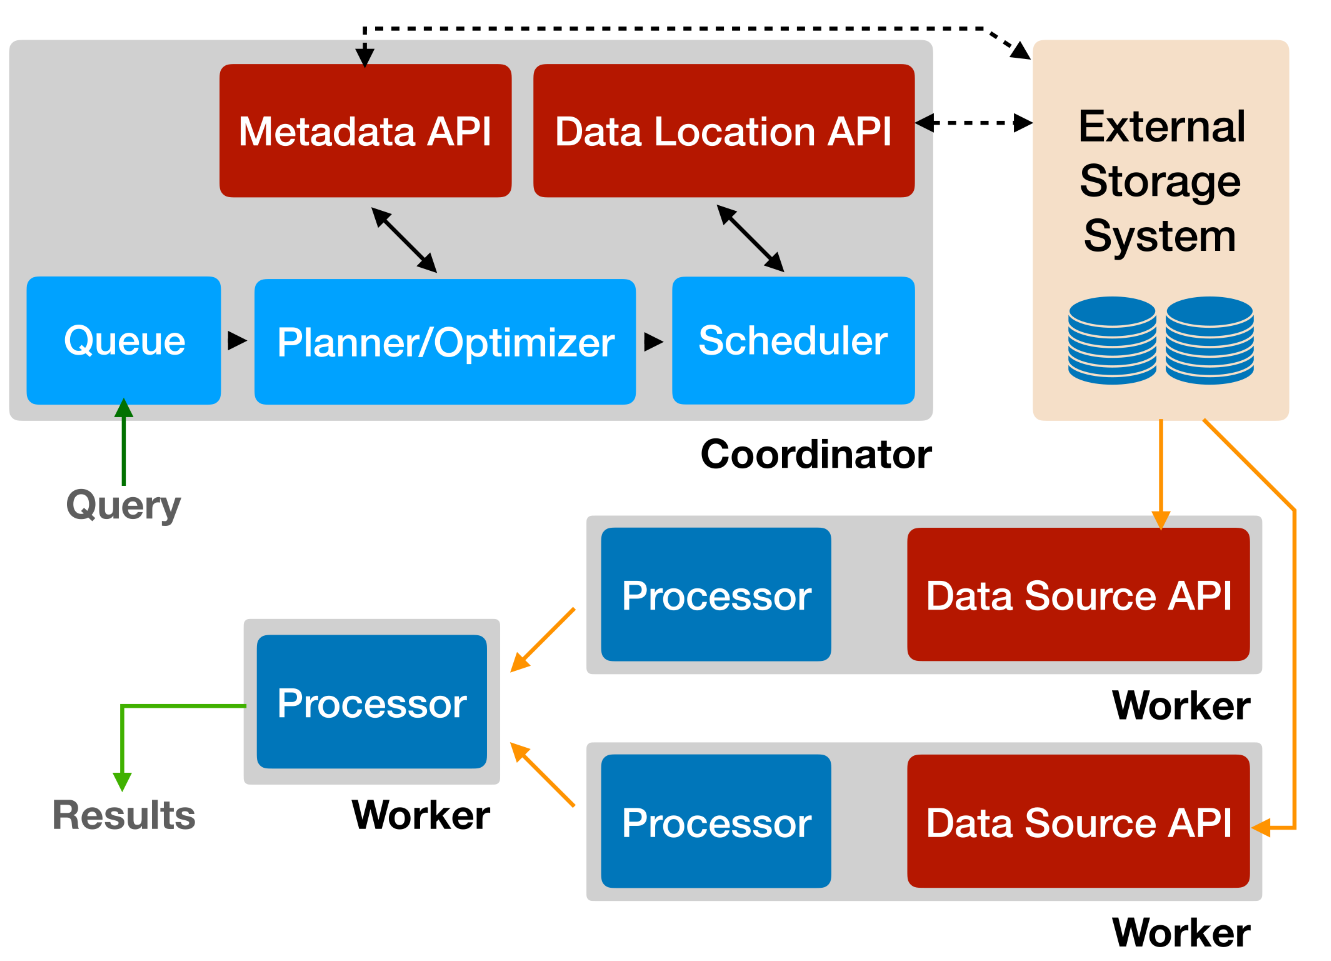
\includegraphics[width=\linewidth, keepaspectratio]{figures/presto-architecture.png}
    \caption{Presto Architecture \cite{b3}}
    \label{fig:presto-arch}
\end{figure}

Presto also offers a plugin interface that allows developers to extend it with custom data types, functions, access control implementations, event consumers, queuing policies, and configuration properties. Among these, the most crucial plugins are the connectors. The connectors enable Presto to connect with various external data stores through the Connector API, which is organized into four components: the Metadata, Data Location, Data Source, and Data Sink APIs. These APIs together support efficient connector implementations in a distributed execution environment.

\subsubsection{Node Types}

The \textit{coordinator} in a Presto cluster serves as the central node, the “brain” of the system, and is responsible for parsing SQL statements, generating query execution plans, handling the worker nodes and monitoring their activity, and orchestrating query execution across the cluster. It is also the endpoint through which clients submit their queries. Every Presto deployment requires one coordinator along with one or more worker nodes, although in a testing or development environment, a single Presto node can be configured to act as both the coordinator and a worker. The query execution process begins with the coordinator, which constructs a logical representation of the query, organizes it into multiple stages, and translates these stages into a set of interconnected tasks that are distributed among the workers.

Presto \textit{workers} are responsible for task execution and data processing. They retrieve data through connectors and exchange intermediate data with each other during query execution. The coordinator collects the data produced by the workers and delivers the final results to the client. When a worker node is launched, it registers itself in the cluster by advertising its presence to the coordinator’s discovery service, thereby becoming available for task assignment. Communication between workers and the coordinator, as well as among workers themselves, is performed through a REST API.


\subsubsection{Components}

A \textit{connector} in Presto is a plug-in that connects the Presto engine to an external catalog. It enables Presto to interact with a wide variety of data sources  for both reading and writing data, including relational databases, NoSQL databases, and filesystems. The connector’s role is to provide Presto with metadata, such as schemas, tables, and column definitions, and map the data from the external source into Presto’s data types. \cite{b4}

A \textit{catalog} represents a data source through its associated connector and contains one or more schemas. Each catalog is bound to a specific connector, and a query execution may operate across multiple catalogs. Catalogs are defined via properties files located in the configuration directory of each Presto node.

A \textit{schema} is used to organize tables within a catalog. Together, a catalog and schema define the set of tables that can be queried \cite{b2}. When accessing various data sources, a schema may either correspond to the same concept in the target database or, depending on the connector, organize the tables according to the data structure of the underlying source.

A \textit{table} in Presto, just like in a relational database, contains a set of rows, each arranged into named columns with associated data types. The way source data is represented as tables is determined by the connector.


\subsubsection{Query Execution Model}

Presto executes ANSI-compatible SQL statements by translating them into queries and devising a query plan that is then distributed across the worker nodes of the cluster.
\newline \indent In Presto, a \textit{statement} simply refers to the textual representation of a SQL query, which consists of clauses, expressions, and predicates.
A \textit{query} refers to the ensemble of components and configurations required to execute a statement, including stages, tasks, splits, connectors, and associated data sources, all working together to produce a result.

A \textit{query plan} outlines the sequence of steps required to retrieve and process data as specified in the SQL query \cite{b2}. It is structured as a tree of nodes, with each node representing an operator. Since SQL is declarative, multiple query plans can be devised to execute a given query, which may vary in performance. So, Presto relies on a query optimizer to select the most efficient one.
Presto’s \textit{query optimization} consists of two phases: logical and physical \cite{b2}. In the logical phase, the plan is refined by focusing exclusively on reducing the algorithmic complexity. Then, in the physical phase, the logically optimized plan is tailored for distributed execution by determining which Presto nodes will execute the query plan and the data exchange strategy between them.

When executing a query, Presto organizes the process into a hierarchy of \textit{stages} that form a tree-like structure. Each query has a root stage that collects and aggregates the results from other stages. While the stages define the distributed query plan, they are not executed directly on workers.
A \textit{stage} is executed as a collection of tasks distributed across the cluster’s worker nodes. Tasks serve as the core processing units within the architecture and operate on splits of data. The stages at the lowest level of a distributed query plan retrieve data through \textit{splits} provided by connectors, while intermediate stages consume data produced by preceding stages. During query scheduling, the Presto coordinator requests a list of all available splits for a table from the connector, tracks which tasks are processing those splits, and on which worker nodes they are running.
Essentially, the distributed query plan is first divided into stages, which are then further broken down into tasks that act upon or process these splits.  Each task has inputs and outputs and runs in parallel with other tasks, which in turn rely on multiple drivers for concurrent execution.
A \textit{driver} is the smallest unit of parallel execution in Presto, and it represents a pipeline of operator instances. Each driver consumes data, produces output by combining its operators, which is then aggregated by a task and forwarded to another task in another stage using an exchange client \cite{b2}.
An \textit{operator} is a processing unit that consumes data, performs a specific operation, such as filtering, projection, or joining, and emits results to be consumed by the next operator in the sequence.


\subsubsection{Query Optimization techniques}

When the Presto coordinator receives a new query from a client, it initiates the query optimizer in order to determine the most efficient execution strategy for the query. It does so by iteratively applying transformation rules until the optimal execution plan is found.\cite{b3,b4} Presto supports three query optimization strategies: predicate pushdown, cost-based optimization, and history-based optimization:

\textit{Predicate pushdown} \\
Predicate pushdown involves moving (``pushing down'') query predicates as close as possible to the data source. As a result, unnecessary data reads are minimized, thereby reducing I/O operations and network traffic, and improving query execution times. This strategy is particularly beneficial for queries involving joins with WHERE clauses, allowing Presto to filter unnecessary data before joining tables.\cite{b4}

\textit{Cost-based optimization (CBO)} \\
CBO is a strategy that evaluates query execution plans based on estimated computational costs. It relies on the table statistics, such as row counts and average column sizes, and leverages this information to determine the most effective join ordering strategy.\cite{b4}

\textit{History-based optimizations (HBO)} \\
HBO is a framework that records statistics from executed queries to reuse them for future queries with similar plans. To identify similar queries, each query plan is canonicalized to eliminate irrelevant differences, such as the naming of intermediate variables, and each plan node is hashed to a string value. Historical statistics associated with the same hash are then applied in HBO. These statistics are preferred over cost-based estimations, with the optimizer falling back to cost-based statistics when historical data is unavailable.\cite{b2}

Note that the connectors for Cassandra, PostgreSQL, and MongoDB do not support providing table statistics, which means that, in our case, Presto cannot utilize the CBO and HBO query optimization techniques.

\subsection{PostgreSQL}

PostgreSQL is an open-source object-relational database system or ORDBMS in abbreviation form \cite{b5}. It was the outcome of the adding of the SQL language, in 1994, to the original POSTGRES package developed at the University of California, Berkeley. After more than three decades of its release, it has elevated itself as one of the most popular database management systems being used by large organizations; including Apple, Reddit and Instagram \cite{b6}, largely because of its characteristics, briefly, mentioned below:

As mentioned, PostgreSQL belongs to the ORDBMS family; thus, it adheres to the ACID properties. This stands for Atomicity, Consistency, Integrity, and Durability – a set of fundamental principles of relational database systems that ensures transaction integrity and data reliability \cite{b7, b8}.

At the same time, PostgreSQL is praised for its implementation of Multi-Version Concurrency Control (MVCC). This system allows concurrent transactions to access the same data without blocking one another. This feature renders PostgreSQL a very valuable tool especially for maintaining high performance in environments with many simultaneous users \cite{b6}.

Flexibility and extensibility constitute another highly sought after property. PostgreSQL is fairly versatile and enables developers to add new database functionality and packets without forking from the original project. Therefore, besides the native standard SQL data types, it has come to additionally support arrays, JSON/JSONB for semi-structured data, and, even, geospatial data \cite{b6,b9,b10}.

Finally, PostgreSQL uses vacuuming to manage storage overhead caused by multiple row versions, while, also, offering advanced query optimization through the usage of various indexing options; including B-Tree, GiST, GIN, and BRIN \cite{b6}.

This rich set of features, query capabilities and transaction management, however, does not come without its drawbacks. The need for query optimization produces inefficiencies in big data storage, and the suboptimal execution of certain types of transactions and join operations. The search for a solution to these problems has led to the emergence of the NoSQL database paradigm, which both MongoDB and Apache Cassandra belong to \cite{b11}.


\subsection{MongoDB}

MongoDB is an open-source NoSQL database developed by 10gen in 2007 in C++. It can be characterized as a Document Store – a type of NoSQL databases. In this context, a document, basically, constitutes a record – a data structure composed of field value pairs. The type of documents used varies by vendor, but it is always defined by known standards, like XML and JSON. MongoDB, in particular, uses the latter \cite{b5, b11, b12}.

MongoDB, though non-relational, it yet implements many features common in relational databases, such as sorting, indexing, range queries and nested document queries \cite{b5}. Therefore, it inherits various advantages from both systems.

To begin with, MongoDB supports embedded data models including documents and arrays. This, combined with the implementation of indexes for faster queries, leads to higher performance through the reduction of the I/O activity on the database system. On the same time, it provides rich query language capabilities in its users by handling both read and write operations, as well as data aggregation and text search. It ensures high availability by providing automatic failover and data redundancy across multiple servers, while, lastly, incorporating horizontal scalability through “sharding” – a process that distributes data across clusters of machines, thereby enhancing both performance and system capacity \cite{b12}.

The aforementioned set of features renders MongoDB a valuable compromise between efficient data storage and query execution. However, there are serious drawbacks that one must consider. Being a NoSQL database forces MongoDB to adhere to the CAP theorem. Theorised in 2000 by Brewer \cite{b13} and formally proved two years later by Gilbert and Lynch \cite{b14, b15}, it stands for Consistency, Availability, and Partition tolerance and it states that it is impossible for a distributed computing system to simultaneously provide all three guarantees. The choice of which feature to discard determines the nature of the system. MongoDB – among others – sacrifices consistency to get a scalable, simple, and high-performance database management system. Furthermore, since MongoDB is denormalized, it doesn’t need to follow a strict relational schema. While this allows for greater flexibility it forces more schema based design decisions on the app logic than the database itself \cite{b7, b12}.


\subsection{Apache Cassandra}

Cassandra is an open-source, highly scalable, distributed NoSQL developed by Apache Software Foundation and written in Java \cite{b11, b16}. Contrary to MongoDB, Cassandra belongs to another type of NoSQL databases; that of Column stores. That is the type most similar to the traditional relational database model, where the column represents the unit of data identified by key and value. The main difference is that Cassandra retains much schema flexibility, being able to also handle semi-structured and unstructured data \cite{b11}.

However, perhaps the most highly sought after feature Cassandra displays is that it is, in fact, designed to handle the storage of large amounts of data and the execution of millions of operations per day. It follows a peer-to-peer strategy, where data can be distributed all over the world, deployed across multiple nodes/data centres. When a node is added or removed, all data is automatically redistributed allowing the failed node to be replaced with no downtime.

Durability is yet another strong point. Cassandra supports two different replication types: synchronous and asynchronous, with the user being able to opt which one to use. A commit log is used to capture all writes and redundancies in order to ensure data durability.

Additionally, Cassandra makes usage of indexing. Each node maintains all indexes of the tables it manages. It is, however, crucial to note that with larger data volumes and unique values, the amount of overhead created by the management of indexes is suboptimal \cite{b11}.

Cassandra’s flexible data model, no single point of failure and linear scalability has rendered it ideal for video streaming services, like Netflix; but, also, for organizations with the need of big data management, including Apple, Facebook, IBM, Instagram, Rackspace, Twitter, Uber, Spotify, Cisco, eBay, etc. \cite{b17}.



\subsection{TPC-DS Benchmark}\label{tpcds}

The TPC-DS benchmark is a standard tool for measuring the performance of a decision support system. It achieves this by providing a set of SQL queries that can be executed on different systems to evaluate and compare their performance \cite{b5}.

This benchmark simulates a real-world business environment by employing large datasets and complex queries to assess how effectively a system can answer critical business questions, analyze trends, and manage data maintenance. To ensure applicability in real-world scenarios, TPC-DS defines 99 distinct SQL queries that cover a wide range of business analysis tasks \cite{b6}.

\subsubsection{Business Model}

TPC-DS models industries that manage, sell, and distribute a wide variety of products such as food, electronics, furniture, music, and toys. It adopts the business model of a large retail enterprise with multiple sales channels (physical stores, mail-order catalogs, and the internet), thus providing a realistic context.

The model not only provides tables for simulating sales and returns but also includes basic inventory management and promotional systems. The benchmark focuses on key business processes, which include:
\begin{itemize}
    \item Recording customer purchases and tracking returns across all sales channels.
    \item Modifying prices according to promotions.
    \item Maintaining warehouse inventory.
    \item Creating dynamic web pages.
    \item Maintaining customer profiles (Customer Relationship Management).
\end{itemize}

\subsubsection{Logical Database Design}

The logical database design of TPC-DS is centered around a snowflake schema, reflecting the complexity of a large retail enterprise. At its core are seven fact tables that capture the primary business processes of the benchmark:
\begin{itemize}
    \item \texttt{store\_sales} and \texttt{store\_returns}: purchases and returns from physical stores.
    \item \texttt{catalog\_sales} and \texttt{catalog\_returns}: purchases and returns from mail-order catalogs.
    \item \texttt{web\_sales} and \texttt{web\_returns}: purchases and returns through the online channel.
    \item \texttt{inventory}: modeling stock for the catalog and online channels.
\end{itemize}

In addition, the schema incorporates 17 dimension tables that provide descriptive context for the fact tables. These dimensions are shared across all sales channels and include details such as customer information, product attributes, time and date of transactions, and more.

Figures 2--8 illustrate the Entity-Relationship (ER) diagrams for each of the seven fact tables as provided by the TPC-DS Standard Specification \cite{b5}.

\begin{figure}[htbp]
    \centering
    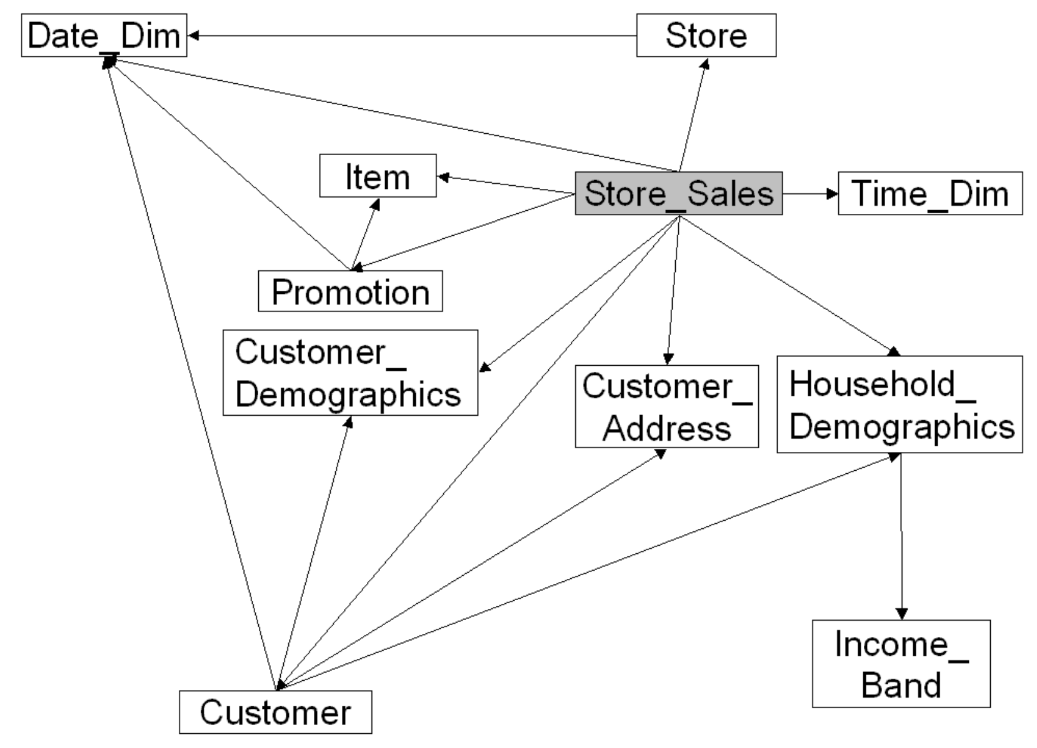
\includegraphics[width=\linewidth]{figures/fact_table_store_sales.png}
    \caption{ER Diagram of \texttt{store\_sales} fact table }
    \label{fig:store_sales}
\end{figure}

\begin{figure}[htbp]
    \centering
    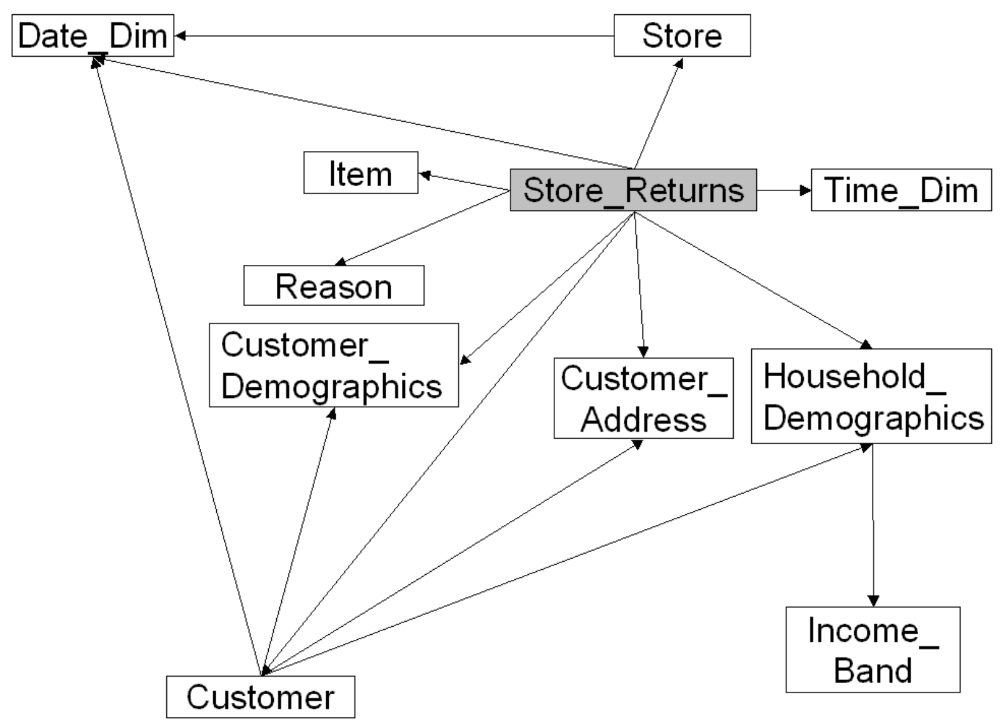
\includegraphics[width=\linewidth]{figures/fact_table_store_returns.png}
    \caption{ER Diagram of \texttt{store\_returns} fact table }
    \label{fig:store_returns}
\end{figure}

\begin{figure}[htbp]
    \centering
    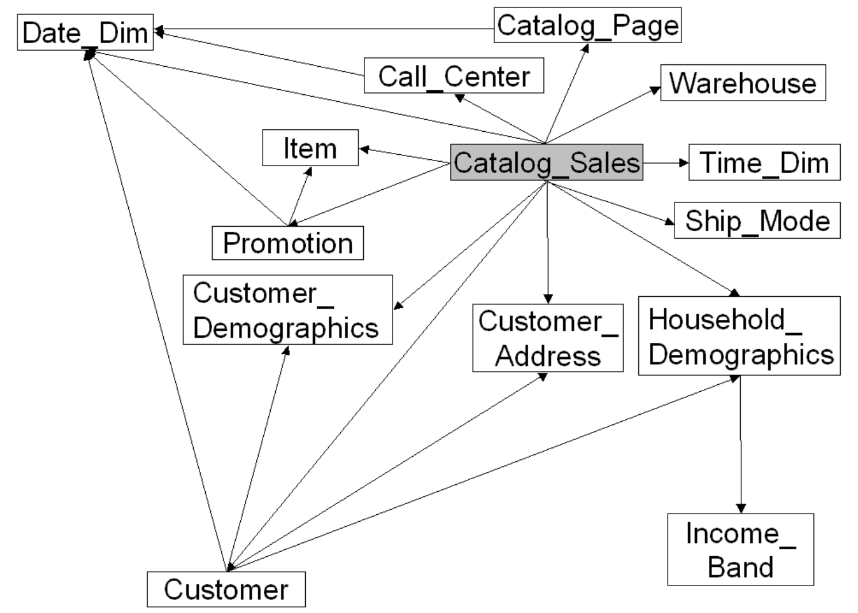
\includegraphics[width=\linewidth]{figures/fact_table_catalog_sales.png}
    \caption{ER Diagram of \texttt{catalog\_sales} fact table }
    \label{fig:catalog_sales}
\end{figure}

\begin{figure}[htbp]
    \centering
    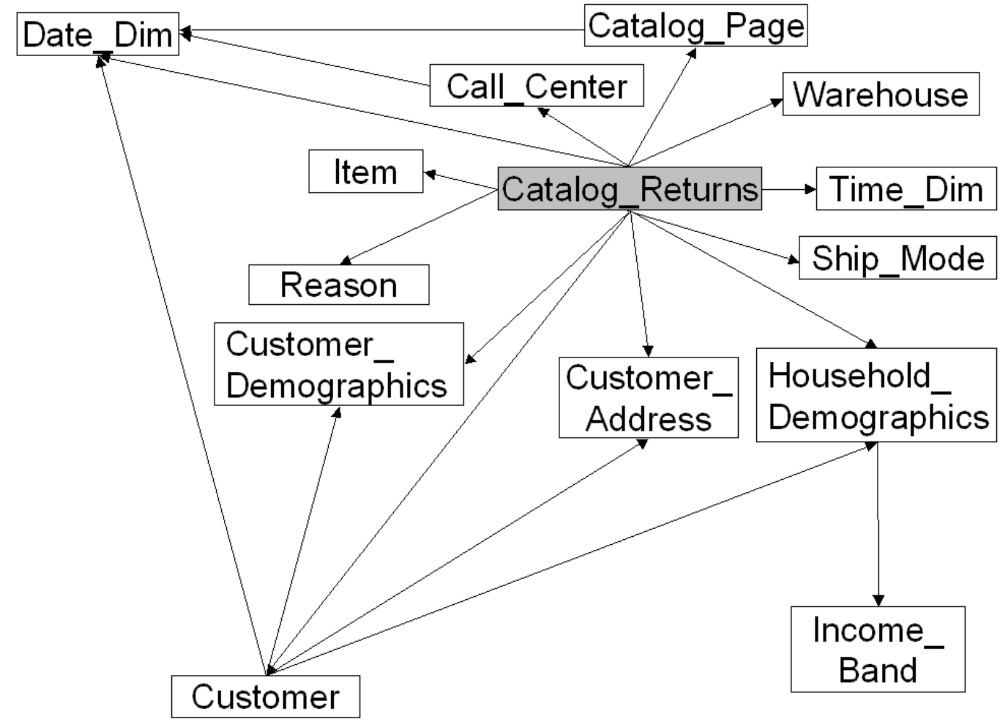
\includegraphics[width=\linewidth]{figures/fact_table_catalog_returns.png}
    \caption{ER Diagram of \texttt{catalog\_returns} fact table }
    \label{fig:catalog_returns}
\end{figure}

\begin{figure}[htbp]
    \centering
    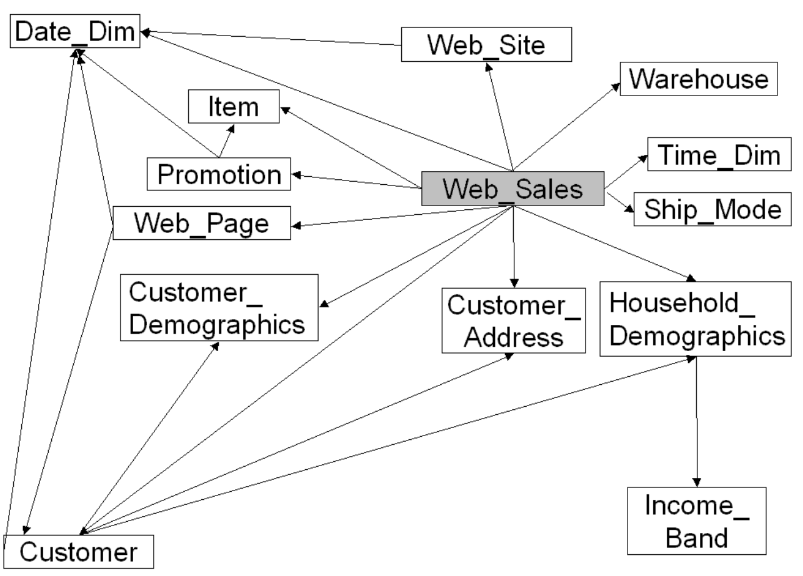
\includegraphics[width=\linewidth]{figures/fact_table_web_sales.png}
    \caption{ER Diagram of \texttt{web\_sales} fact table }
    \label{fig:web_sales}
\end{figure}

\begin{figure}[htbp]
    \centering
    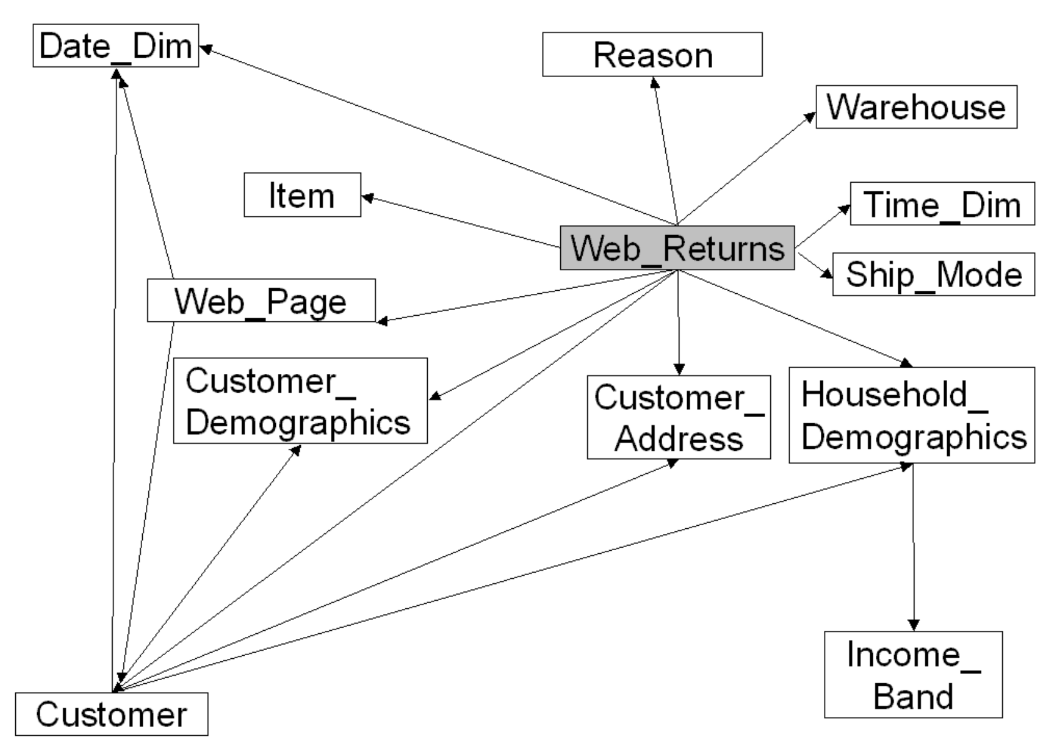
\includegraphics[width=\linewidth]{figures/fact_table_web_returns.png}
    \caption{ER Diagram of \texttt{web\_returns} fact table }
    \label{fig:web_returns}
\end{figure}

\begin{figure}[htbp]
    \centering
    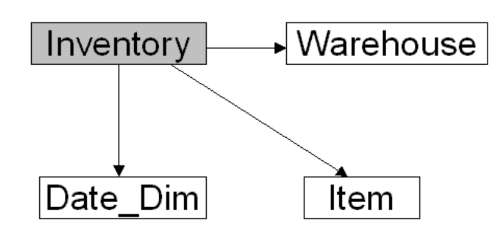
\includegraphics[width=\linewidth]{figures/fact_table_inventory.png}
    \caption{ER Diagram of \texttt{inventory} fact table }
    \label{fig:inventory}
\end{figure}

\subsubsection{Query Classes}

The TPC-DS benchmark provides a set of queries that we used to design the appropriate data distribution strategy. These queries can be classified into four main categories, based on the type of user and the information they are intended to retrieve from the decision support system:

\begin{itemize}
    \item \textbf{Reporting queries:} Queries that answer pre-defined questions, often with minor variations such as date range or location.
    \item \textbf{Ad hoc queries:} Queries that dynamically answer immediate and specific business questions, in contrast to the pre-planned nature of reporting queries.
    \item \textbf{Iterative OLAP queries:} Queries aimed at exploring and analyzing data to discover new relationships and trends.
    \item \textbf{Data mining queries:} Queries that sift through large amounts of data to uncover relationships and predict future trends, typically involving large joins and aggregations. \cite{b5}
\end{itemize}

\section{Source Code}\label{source_code}

All configuration files, scripts, and guidelines required to set up the Presto cluster are available in a dedicated GitHub repository. This repository serves as a complete reference for reproducing the cluster environment, including the installation and configuration of PrestoDB, instructions for installing the database management systems, generating the TPC-DS benchmark data, and importing it into the databases.

The repository can be accessed at the following link:

\begin{center}
    \href{https://github.com/mpantelakis/ntua-info-systems}{GitHub Repository}
\end{center}


\section{Installation and Configuration}

\subsection{PrestoDB Cluster Setup}

Due to the limited available resources, we cannot create a Presto cluster with multiple workers, where each functions as an independent computing node. Therefore, to make full use of the available resources, the workers must be treated as processes on the same machine, sharing its resources in a way that simulates independent compute nodes (where feasible). To this end, we have distributed the 16 total CPU cores of the two machines between the coordinator and three workers. Using the Linux \texttt{taskset} command, we have assigned each process to a specific 4-core set. The coordinator and first worker share the first machine's cores, and the other two workers share the second machine's cores. Additionally, we have limited the total available memory for each node to 4 GB through the JVM configuration file.

Regarding the database systems, due to the high memory requirements of the Cassandra system, we have chosen to install it alone on the first machine, while MongoDB and PostgreSQL are installed on the second machine. Figure~\ref{fig:cluster_topology} illustrates the overall topology of the cluster.

\begin{figure}[htbp]
    \centering
    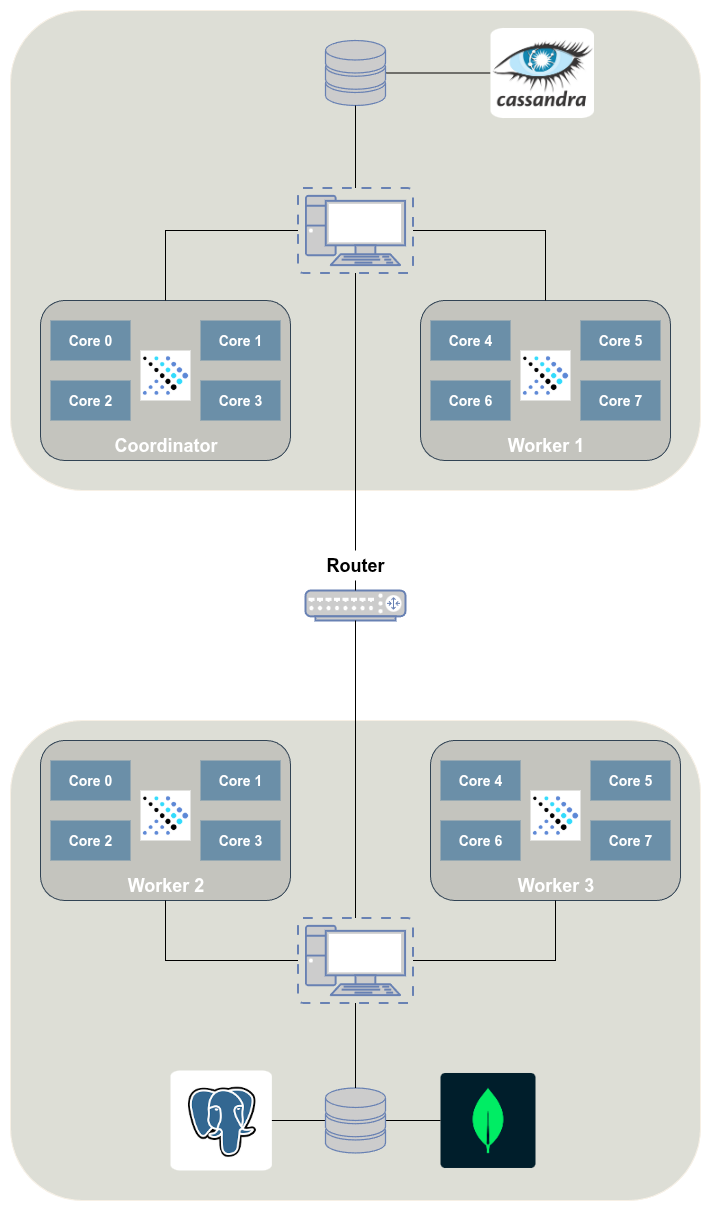
\includegraphics[width=\linewidth]{figures/cluster_topology.png}
    \caption{PrestoDB Cluster Topology }
    \label{fig:cluster_topology}
\end{figure}

It is clear that the network connectivity between the machines is not ideal, as they do not belong to the same subnet. Consequently, data transfers between the nodes are subject to potential delays, making the cluster's performance highly dependent on the available network bandwidth and latency.

\subsection{PrestoDB Nodes Configuration}

Each Presto node resides within its own Presto installation folder. Within this folder, it is necessary to define the \texttt{etc} directory, which contains the following configuration files:

\begin{itemize}
    \item \textbf{Node Properties} (\texttt{node.properties}): Specifies environment-specific settings for each Presto node, such as the node ID.
    \item \textbf{JVM Config} (\texttt{jvm.config}): Contains command-line options for the Java Virtual Machine running the Presto node.
    \item \textbf{Config Properties} (\texttt{config.properties}): Defines Presto server configurations, including coordinator/worker settings and query-related parameters.

    \item \textbf{Log Properties} (\texttt{log.properties}): Configures logging for the Presto node, including log levels and format.
\end{itemize}


Inside the \texttt{etc} directory, there must also be a \texttt{catalog} directory containing all the connectors, one for each database system (e.g., \texttt{cassandra.properties}, \texttt{mongodb.properties}, \texttt{postgresql.properties}).

Finally, within the installation folder, it is necessary to create the \texttt{data} directory, which will store all log files.


\subsection{TPC-DS Benchmark Data \& Queries Generation}

The TPC-DS Benchmark Suite provides the capability to generate data through the tool \texttt{dsdgen}. It produces data by taking as main parameters the scale factor, i.e., the total size of the data in GB to be generated, and the output directory. Below is an example execution of \texttt{dsdgen} for generating data with a total size of 1GB:

\begin{verbatim}
dsdgen -scale 1 -dir /home/user/tpcds-data
\end{verbatim}

To determine the total data size to be generated, we had to account for the limited storage available, which was further constrained by PostgreSQL and MongoDB sharing the same storage device. As mentioned in Section~\ref{no_dist}, the base benchmarks required loading the entire dataset into each database system, which created an additional limitation. After testing, we selected a total data size of 8 GB. It is worth noting that, although the overall dataset size was 8.6 GB, the actual storage occupied by each system varied. Specifically, the observed data sizes in each system were:

\begin{itemize}
    \item Cassandra: 5.9 GB
    \item MongoDB: 10.58 GB
    \item PostgreSQL: 17 GB
\end{itemize}


In addition to data generation, the TPC-DS Benchmark Suite also offers 99 query templates for benchmarking purposes. These templates can be converted into executable SQL queries using the tool \texttt{dqgen}. In Section~\ref{query_selection}, we describe the process of selecting some of these queries to use in our benchmarks.


\subsection{Data Population of Database Systems}

To load the generated data into the three database systems, we created two Bash scripts,
one for Cassandra and one for PostgreSQL, and a Python script for MongoDB.

For Cassandra, we used the native client \texttt{cqlsh} with the \texttt{COPY} command.
For PostgreSQL, we used its native client as well.

However, for MongoDB we did not use the official data import tool, \texttt{mongoimport},
since it does not support the ``\texttt{|}'' delimiter (used by TPC-DS when generating data).
Instead, we developed a Python script using the \texttt{pymongo} library.

All three scripts are available in the GitHub repository referenced in Section~\ref{source_code}.

\section{Benchmark Query Selection and Classification}\label{query_selection}

We selected a subset of 28 out of the 99 total queries. The selection was done carefully, checking that all fact tables were used and having both a structural and a logical variety in each single query. The queries were then organized into two main dimensions: their complexity and the number of fact tables accessed within the query.

Within these dimensions, we created five groups in total: three focused on complexity, and two related to the number of fact tables used. Specifically:

\begin{enumerate}
    \item \textbf{Complexity Classification:} The 28 queries were split into three categories based on their structural complexity:
          \begin{itemize}
              \item \textit{Simple Complexity:} The queries in this category are characterized by basic operations along with simple aggregation functions, without the use of advanced subqueries or complex Common Table Expressions (CTEs).
              \item \textit{Medium Complexity:} The queries in this category are characterized by a more advanced structure, with numerous aggregations and complex logic through the use of nested subqueries and CTEs.
              \item \textit{High Complexity:} The queries in this category are characterized by a high degree of complexity. They feature multiple CTEs, extensive use of nested subqueries, and complex join operations.
          \end{itemize}
    \item \textbf{Fact Table Access Classification:} The 28 queries were split into two groups based on the number of fact tables they interact with:
          \begin{itemize}
              \item \textit{Single Fact Table:} The queries in this category access only one fact table.
              \item \textit{Multiple Fact Table:} The queries in this category access multiple fact tables.
          \end{itemize}
\end{enumerate}

So, the total of 5 groups allowed us to gain a whole view of the 3 DBMS we had and how each change affected the whole system. In this way, we can design the appropriate data distribution strategy to maximize the system’s performance.

The selected queries and their categorization into respective groups are shown in Table~\ref{tab:query_groups}.

\begin{table}[h!]
    \centering
    \renewcommand{\arraystretch}{1.3}
    \caption{Categorization of the selected TPC-DS queries}
    \begin{tabular}{|>{\centering\arraybackslash}c|>{\centering\arraybackslash}m{6cm}|} % use m{6cm} for vertical centering
        \hline
        \textbf{Group}               & \textbf{Queries}                                                         \\
        \hline
        \textbf{Simple Complexity}   & 1, 2, 7, 14, 15, 16, 20, 23, 32                                          \\
        \hline
        \textbf{Medium Complexity}   & 5, 8, 12, 13, 17, 21, 22, 24, 39, 94                                     \\
        \hline
        \textbf{High Complexity}     & 3, 4, 6, 9, 10, 30, 37, 48, 49                                           \\
        \hline
        \textbf{Single Fact Table}   & 1, 2, 4, 5, 7, 8, 12, 13, 14, 15, 16, 21, 23, 24, 30, 32, 37, 39, 49, 94 \\
        \hline
        \textbf{Multiple Fact Table} & 3, 6, 9, 10, 17, 20, 22, 48                                              \\
        \hline
    \end{tabular}
    \label{tab:query_groups}
\end{table}

Note that, in order to implement an effective data distribution strategy, we carefully selected a set of queries from all four categories described in Section~\ref{tpcds} to ensure that the system’s performance would be both optimal and representative across the full range of real-world business intelligence tasks \cite{b5}.

\section{Data Distribution Strategies and Results Analysis}

 [A short intro for the section]

\subsection{No Data Distribution Applied}\label{no_dist}

For our first experiment, we measured the performance of every database management system independently from one another; without implementing any form of data distribution. This decision was made in order to test in practice their strengths and weaknesses, as they were discussed in Section~\ref{SystemArchitecture}, to view how they handle different query operations and needs, and, in general, to establish a baseline understanding of each DBMS. To this end, we ran – with a single worker at a time – each group’s queries five times for every DBMS and we recorded the execution time. Afterwards, we calculated the arithmetic means of the execution times per query for every group and plotted them. The results of this process are shown in Figure~\ref{fig:no_dist_applied}.

\begin{figure}[htbp]
    \centering
    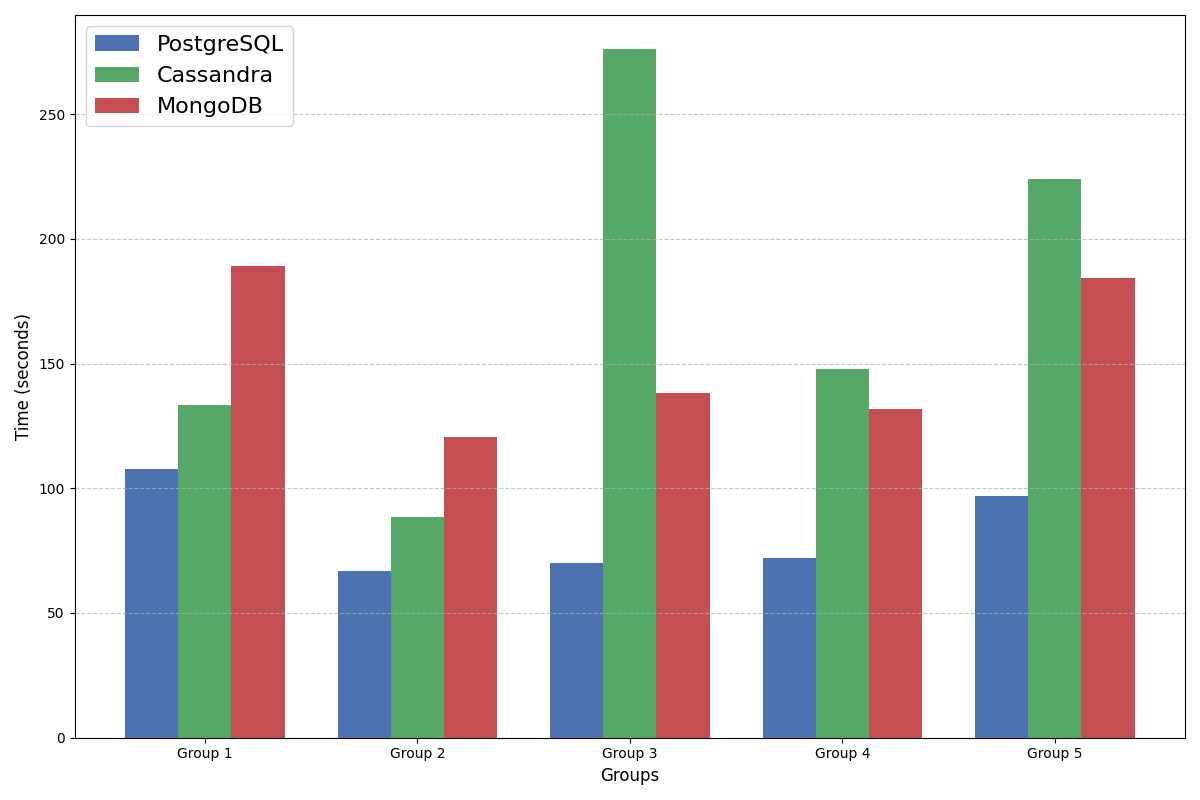
\includegraphics[width=\linewidth]{figures/no_dist_applied.png}
    \caption{Average Execution Time by Group and Database System - No Distribution Applied}
    \label{fig:no_dist_applied}
\end{figure}

The first thing to notice is that PostgreSQL achieves steadily lower query execution times relatively to the other two database systems across all five groups. This confirms the theoretical superiority of object-relational database systems regarding query execution performance. However, it must be reminded that despite its high operation efficiency, PostgreSQL lacks in data storage efficiency.

Regarding the two NoSQL databases – MongoDB and Cassandra – the results are less straightforward. As the complexity of the queries remains relatively low for the first two groups, Cassandra achieves lower execution times than MongoDB; it is around 40\% quicker. However, for group 3, we have a completely different image. Cassandra seems incapable of handling the high complexity and large computational resources needed from the queries involved. It lacks efficient support for ad-hoc or multi-dimensional queries. On the contrary, MongoDB gains heavily from the way it organizes its data and its indexing strategies, enabling it to handle a broader range of query patterns more gracefully.

For group 4, the same trend continues, while for group 5, Cassandra, once more, appears more efficient than MongoDB. This seems paradoxical at first given that group 5 contains queries handling multiple fact tables, and, thus, larger amount of data. However, after a closer examination, one can notice that the queries of group 5 contain less direct join operations, and despite the fact that they span multiple fact tables, those are handled as independently, as different subqueries, causing Cassandra to, contradictorily, outperform MongoDB.

To conclude the results from the first experiment with no data distribution, PostgreSQL appears to be the most reliable across all query groups. Cassandra and MongoDB exhibit mixed results; however the performance collapse of the former for queries of higher complexity will be taken into consideration moving to the next data distribution strategies.


\subsection{Fact Table Size \& ER Based Distribution}

We based the first method of distributing the data across the three systems solely on the size of the fact tables and the previous results regarding the overall performance of each system. Initially, we sorted the fact tables in descending size order, as shown in Table~\ref{tab:fact_table_sizes}, based on the size of the data files generated by TPC-DS for each table.

\begin{table}[h!]
    \centering
    \renewcommand{\arraystretch}{1.2}
    \caption{Sizes of TPC-DS fact tables}
    \begin{tabular}{|l|c|}
        \hline
        \textbf{Fact Table} & \textbf{Size} \\
        \hline
        store\_sales        & 3.0 GB        \\
        \hline
        catalog\_sales      & 2.3 GB        \\
        \hline
        inventory           & 1.6 GB        \\
        \hline
        web\_sales          & 1.2 GB        \\
        \hline
        store\_returns      & 256 MB        \\
        \hline
        catalog\_returns    & 168 MB        \\
        \hline
        web\_returns        & 78 MB         \\
        \hline
    \end{tabular}
    \label{tab:fact_table_sizes}
\end{table}


The goal was to assign an appropriate data volume of the fact tables to each system in proportion to its demonstrated performance. PostgreSQL, which demonstrated the best performance, was assigned the largest data volume (store\_sales and catalog\_sales), while MongoDB and Cassandra were assigned smaller data volumes (inventory, web\_sales, store\_returns, catalog\_returns, and web\_returns, respectively). Cassandra naturally handled the smallest volume. The dimension tables appear in each system according to the ER of the fact tables they host. In other words, the dimension tables are duplicated or triplicated within the cluster.
The overall distribution of tables across the three systems is summarized in Table~\ref{tab:table_distribution_1}, while the corresponding benchmarking results are shown in Figure~\ref{fig:dist_method_1}.

\begin{figure}[htbp]
    \centering
    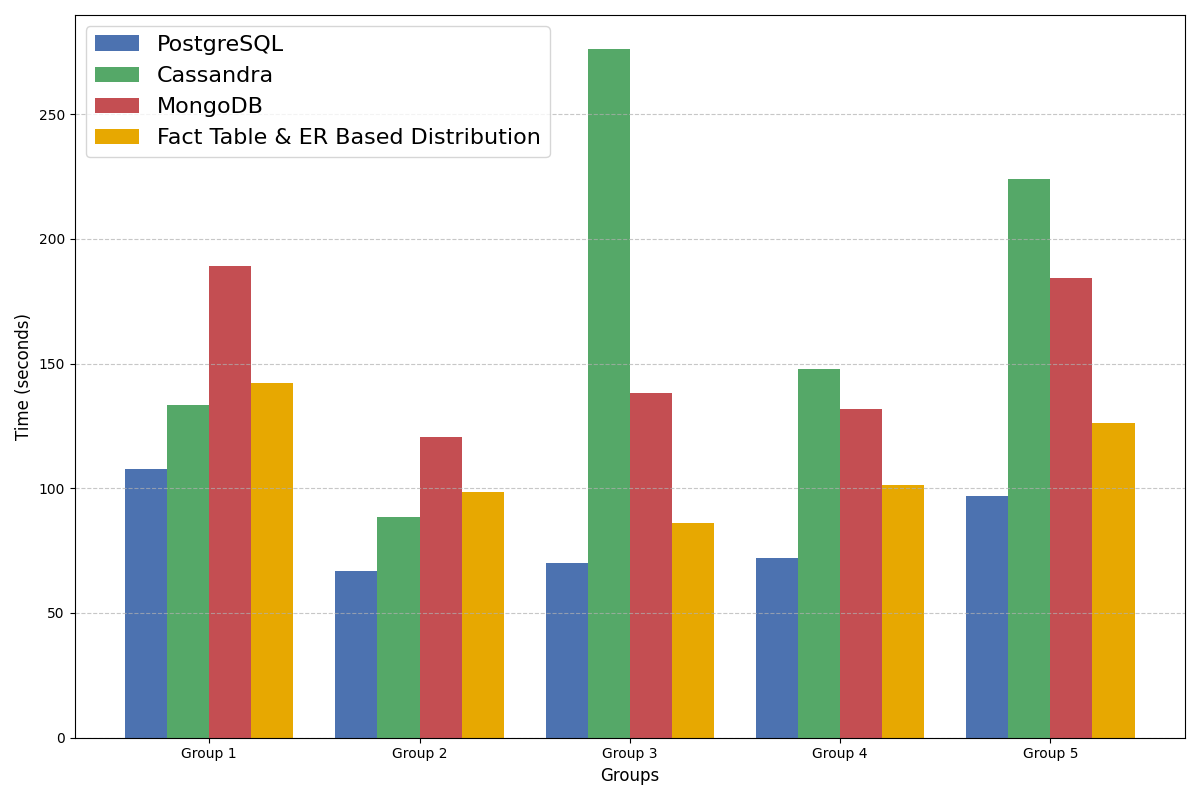
\includegraphics[width=\linewidth]{figures/dist_method_1.png}
    \caption{Average Execution Time by Group - Fact Tables \& ER Based Distribution Method}
    \label{fig:dist_method_1}
\end{figure}


\begin{table}[htbp]
    \centering
    \renewcommand{\arraystretch}{1.2}
    \caption{Fact Table Size \& ER-Based Distribution Method - Data Distribution}
    \resizebox{\linewidth}{!}{%
        \begin{tabular}{|l|c|c|c|}
            \hline
            \textbf{Table}          & \textbf{PostgreSQL} & \textbf{MongoDB} & \textbf{Cassandra} \\
            \hline
            call\_center            & \checkmark          &                  & \checkmark         \\
            \hline
            catalog\_page           & \checkmark          &                  & \checkmark         \\
            \hline
            catalog\_returns        &                     &                  & \checkmark         \\
            \hline
            catalog\_sales          & \checkmark          &                  &                    \\
            \hline
            customer                & \checkmark          & \checkmark       & \checkmark         \\
            \hline
            customer\_address       & \checkmark          & \checkmark       & \checkmark         \\
            \hline
            customer\_demographics  & \checkmark          & \checkmark       & \checkmark         \\
            \hline
            date\_dim               & \checkmark          & \checkmark       & \checkmark         \\
            \hline
            household\_demographics & \checkmark          & \checkmark       & \checkmark         \\
            \hline
            income\_band            & \checkmark          & \checkmark       & \checkmark         \\
            \hline
            inventory               &                     & \checkmark       &                    \\
            \hline
            item                    & \checkmark          & \checkmark       & \checkmark         \\
            \hline
            promotion               & \checkmark          & \checkmark       &                    \\
            \hline
            reason                  & \checkmark          &                  & \checkmark         \\
            \hline
            ship\_mode              & \checkmark          & \checkmark       & \checkmark         \\
            \hline
            store                   & \checkmark          &                  & \checkmark         \\
            \hline
            store\_returns          &                     &                  & \checkmark         \\
            \hline
            store\_sales            & \checkmark          &                  &                    \\
            \hline
            time\_dim               & \checkmark          & \checkmark       & \checkmark         \\
            \hline
            warehouse               & \checkmark          & \checkmark       & \checkmark         \\
            \hline
            web\_page               & \checkmark          & \checkmark       & \checkmark         \\
            \hline
            web\_returns            &                     &                  & \checkmark         \\
            \hline
            web\_sales              &                     & \checkmark       &                    \\
            \hline
            web\_site               & \checkmark          & \checkmark       &                    \\
            \hline
        \end{tabular}%
    }
    \label{tab:table_distribution_1}
\end{table}

Distribution Method 1 (Fact Table \& ER-Based Distribution) achieves execution times between those of PostgreSQL and the NoSQL systems. It does not match PostgreSQL’s single-node performance, but it provides a good balance and demonstrates that distributing based on fact table size \& ER relationships reduces overhead compared to MongoDB and Cassandra individually. The improvement comes mainly from balancing the workload proportionally to each system’s strengths. PostgreSQL was assigned the heaviest fact tables, thereby preventing Cassandra or MongoDB from being overloaded with data volumes that they cannot process effectively. The biggest improvement from Distribution 1 is visible in Group 3 (high-complexity queries), where it clearly outperforms MongoDB and Cassandra by a large margin, though still behind PostgreSQL.


\subsection{Logical Fact Table Pair Distribution}

Designing our second distribution strategy, we kept the same basic principle as before: each fact table was paired with its associated dimension tables, as indicated by the ER diagrams. However, now we also took advantage of the logical relationships between fact tables. Specifically, we noticed that certain fact tables form pairs based on their meaning. A simple example is the pair store\_sales and store\_returns. The logical connection between these tables often makes them appear together in queries. This thought was confirmed through an observation of our query set, which showed that a large proportion followed this pattern. Based on this insight, we adjusted the strategy so that each of these logical pairs was placed in the same DBMS, along with their corresponding dimension tables.

The exact distribution selected in this experiment is shown in Table~\ref{tab:table_distribution_2}.
\begin{table}[htbp]
    \centering
    \renewcommand{\arraystretch}{1.2}
    \caption{Logical Fact Table Pair Distribution Method - Data Distribution}
    \resizebox{\linewidth}{!}{%
        \begin{tabular}{|c|c|c|c|}
            \hline
            Table                   & PostgreSQL & MongoDB    & Cassandra  \\
            \hline
            call\_center            & \checkmark & \          & \          \\
            \hline
            catalog\_page           & \checkmark & \          & \          \\
            \hline
            catalog\_returns        & \checkmark & \          & \          \\
            \hline
            catalog\_sales          & \checkmark & \          & \          \\
            \hline
            customer                & \checkmark & \checkmark & \          \\
            \hline
            customer\_address       & \checkmark & \checkmark & \          \\
            \hline
            customer\_demographics  & \checkmark & \checkmark & \          \\
            \hline
            date\_dim               & \checkmark & \checkmark & \checkmark \\
            \hline
            household\_demographics & \checkmark & \checkmark & \          \\
            \hline
            income\_band            & \checkmark & \checkmark & \          \\
            \hline
            inventory               & \          & \          & \checkmark \\
            \hline
            item                    & \checkmark & \checkmark & \checkmark \\
            \hline
            promotion               & \checkmark & \checkmark & \          \\
            \hline
            reason                  & \checkmark & \checkmark & \          \\
            \hline
            ship\_mode              & \checkmark & \checkmark & \          \\
            \hline
            store                   & \checkmark & \          & \          \\
            \hline
            store\_returns          & \checkmark & \          & \          \\
            \hline
            store\_sales            & \checkmark & \          & \          \\
            \hline
            time\_dim               & \checkmark & \checkmark & \          \\
            \hline
            warehouse               & \checkmark & \checkmark & \checkmark \\
            \hline
            web\_page               & \          & \checkmark & \          \\
            \hline
            web\_returns            & \          & \checkmark & \          \\
            \hline
            web\_sales              & \          & \checkmark & \          \\
            \hline
            web\_site               & \          & \checkmark & \          \\
            \hline
        \end{tabular}
    }
    \label{tab:table_distribution_2}
\end{table}


Figure~\ref{fig:dist_method_2} illustrates the improved performance of the second distribution strategy compared to the first. Notably, the new strategy achieved execution times close to those of a single-node PostgreSQL system, highlighting a significant gain in efficiency. The performance improvement of Distribution 2 (Logical Fact Table Pair Distribution) over Distribution 1 ranges from 15.18\% to 28.9\% across different query groups.

\begin{figure}[htbp]
    \centering
    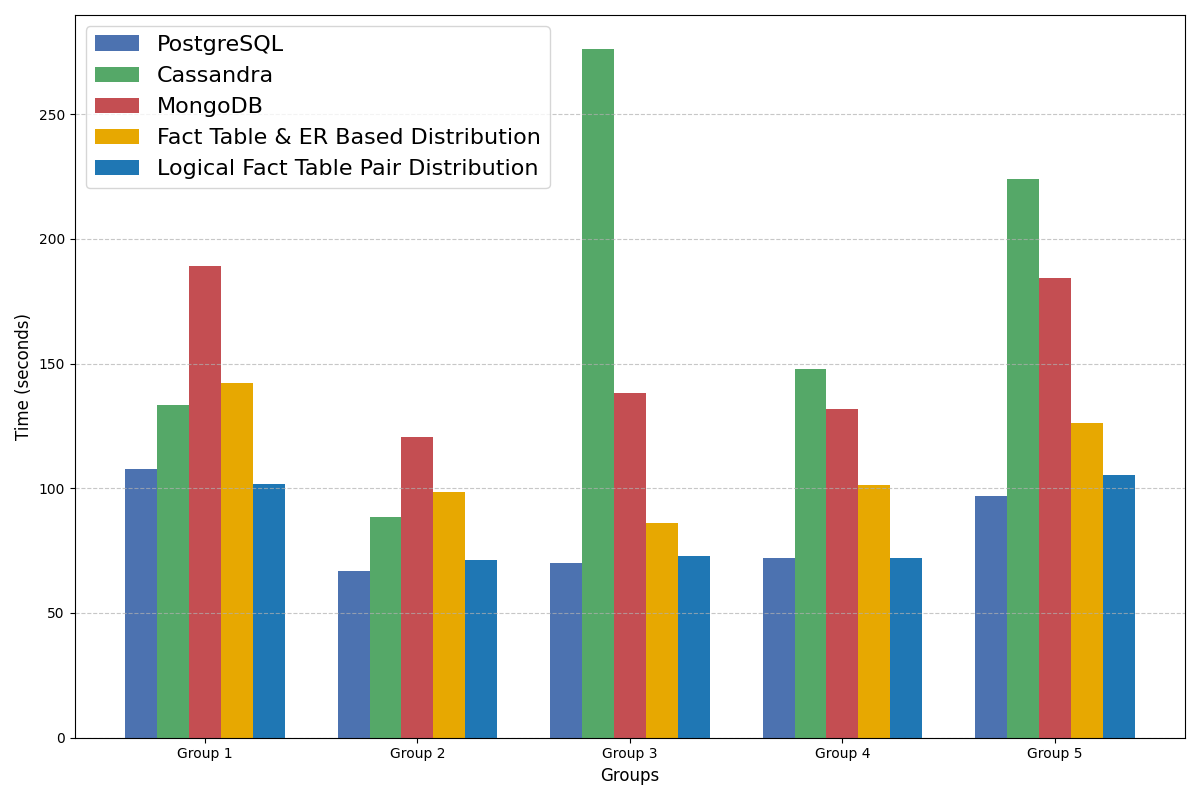
\includegraphics[width=\linewidth]{figures/dist_method_2.png}
    \caption{Average Execution Time by Group - Logical Fact Table Pair Distribution Method}
    \label{fig:dist_method_2}
\end{figure}

The distribution choice of storing logically related fact tables together helped reduce the inter-database communication required for executing queries that involve both fact tables of a pair. By keeping sales-returns fact tables couples within the same DBMS, latency and overhead were significantly reduced leading to a more efficient query execution, with performance approaching that of a non-distributed database.


\subsection{Dimension Table Frequency-Based Distribution}

\subsection{Dimension Table Relationship-Weighted Distribution}

\subsection{Impact of Multi-Worker Execution}

\section{Conclusion}

\begin{thebibliography}{00}
    \bibitem{b1} ``okeanos-knossos IAAS,'' Grnet.gr, 2019.
    \url{https://okeanos-knossos.grnet.gr/}.
    \bibitem{b2} ``Overview - Presto 0.294 Documentation,'' Prestodb.io, 2025. \href{https://prestodb.io/docs/current/overview.html}{https://prestodb.io/docs/current/overview.html}.
    \bibitem{b3} R. Sethi et al., ``Presto: SQL on Everything,''
    2019 IEEE 35th International Conference on Data Engineering (ICDE), Apr. 2019.
    \url{https://doi.org/10.1109/icde.2019.00196}.
    \bibitem{b4} Angelica Lo Duca, T. Meehan, Vivek Bharathan, and Y. Su, Learning and Operating Presto.``O’Reilly Media, Inc.,'' 2023.
    \bibitem{b5} A. Makris, K. Tserpes, G. Spiliopoulos, D. Zissis, and D. Anagnostopoulos, ``MongoDB Vs PostgreSQL: A comparative study on performance aspects,'' \textit{GeoInformatica}, vol. 25, Jun. 2020. doi: \url{https://doi.org/10.1007/s10707-020-00407-w}.

    \bibitem{b6} S. V. Salunke and A. Ouda, ``A Performance Benchmark for the PostgreSQL and MySQL Databases,'' \textit{Future Internet}, vol. 16, no. 10, pp. 382--382, Oct. 2024. doi: \url{https://doi.org/10.3390/fi16100382}.

    \bibitem{b7} S. Juba and A. Volkov, Learning PostgreSQL 11: a beginner’s guide to building high-performance PostgreSQL database solutions, Birmingham, UK: Packt Publishing, 2019.

    \bibitem{b8} GeeksforGeeks, ``ACID Properties in DBMS,'' GeeksforGeeks, Aug. 07, 2016. \url{https://www.geeksforgeeks.org/dbms/acid-properties-in-dbms/}.

    \bibitem{b9} U. Cubukcu, O. A. Erdogan, S. Pathak, S. Sannakkayala, and M. Slot, ``Citus: Distributed PostgreSQL for Data-Intensive Applications,'' in \textit{International Conference on Management of Data}, Jun. 2021. doi: \url{https://doi.org/10.1145/3448016.3457551}.

    \bibitem{b10} PostGIS Developers, ``PostGIS — Spatial and Geographic Objects for PostgreSQL,'' Postgis.net, 2020. \url{https://postgis.net/}.

    \bibitem{b11} V. Abramova and J. Bernardino, ``NoSQL Databases: MongoDB vs Cassandra,'' in \textit{Proceedings of the International C* Conference on Computer Science and Software Engineering - C3S2E ’13}, 2013. doi: \url{https://doi.org/10.1145/2494444.2494447}.

    \bibitem{b12} A. Chauhan, ``A Review on Various Aspects of MongoDb Databases,'' \textit{International Journal of Engineering Research \& Technology}, vol. 8, no. 5, May 2019. \url{https://www.ijert.org/a-review-on-various-aspects-of-mongodb-databases}.

    \bibitem{b13} E. A. Brewer, ``Towards robust distributed systems,'' in \textit{Proceedings of the nineteenth annual ACM symposium on Principles of distributed computing - PODC ’00}, 2000. doi: \url{https://doi.org/10.1145/343477.343502}.

    \bibitem{b14} S. Gilbert and N. Lynch, ``Brewer’s conjecture and the feasibility of consistent, available, partition-tolerant web services,'' \textit{ACM SIGACT News}, vol. 33, no. 2, p. 51, Jun. 2002. doi: \url{https://doi.org/10.1145/564585.564601}.

    \bibitem{b15} S. Gilbert and N. Lynch, ``Perspectives on the CAP Theorem,'' \textit{Computer}, vol. 45, no. 2, pp. 30--36, Feb. 2012. doi: \url{https://doi.org/10.1109/MC.2011.389}.

    \bibitem{b16} G. Wang and J. Tang, ``The NoSQL Principles and Basic Application of Cassandra Model,'' in 2012 \textit{International Conference on Computer Science and Service System}, Aug. 2012. doi: \url{https://doi.org/10.1109/csss.2012.336}.

    \bibitem{b17} H. Tu, ``Cassandra vs. MongoDB: A Systematic Review of Two NoSQL Data Stores in Their Industry Uses,'' in \textit{2024 IEEE 7th International Conference on Big Data and Artificial Intelligence (BDAI)}, Beijing, China, pp. 81--86, Jul. 2024. doi: \url{https://doi.org/10.1109/bdai62182.2024.10692676}.
    \bibitem{b18} ``TPC BENCHMARK\texttrademark DS Standard Specification Version 4.0.0,''
    Transaction Processing Performance Council (TPC), 2024. [Online]. Available: \url{https://www.tpc.org/TPC_Documents_Current_Versions/pdf/TPC-DS_v4.0.0.pdf}
    \bibitem{b19} R. O. Nambiar and Meikel Poess, ``The making of TPC-DS,''
    in \textit{Proceedings of the 32nd International Conference on Very Large Data Bases (VLDB)}, Sep. 2006, pp. 1049--1058.
    doi: \url{https://doi.org/10.5555/1182635.1164217}
\end{thebibliography}

\end{document}
